\section{Directed Team Graph (DiTG)}

In order to measure human workload within the context of our model \cite{gledhill2013modelinguas} we
have defined the following set of core components which allows us to correlate
the activity within our model to human workload.  We call this framework the
directed team graph (DiTG).

\subsection{Conceptual Model}
In previous work we represented WiSAR as a collection of directed role graphs
(DiRGs)\cite{gledhill2013modelinguas}.  See figure~\ref{fig:ditg}.  As is common
when modeling human-automation interaction we have decided to model the DiRGs usings Mealy
state machines~\cite{bolton2013litreview}.  The DiTG formalizes this collection
by defining the communication mediums which unite the said DiRGs.  Using
multiple resource theory\cite{wickens2002multiple} as a guide we can explicitly
define the channels over which this communication occurs.  See
figure~\ref{fig:ditg_detail}.  The Actor state transitions then use these
channels to broadcast and receive inter-Actor communication.  

We hope to gain
insight into decreasing the system workload, and possibly combining roles, by
establishing metrics associated with the task model and model simulation.  These
metrics can then be used to determine if changes to the model represent a
decrease in operator workload.

\begin{figure}
\center
\setlength{\abovecaptionskip}{1mm}
\setlength{\belowcaptionskip}{1mm}
\setlength{\textfloatsep}{1mm}
\setlength{\floatsep}{1mm}
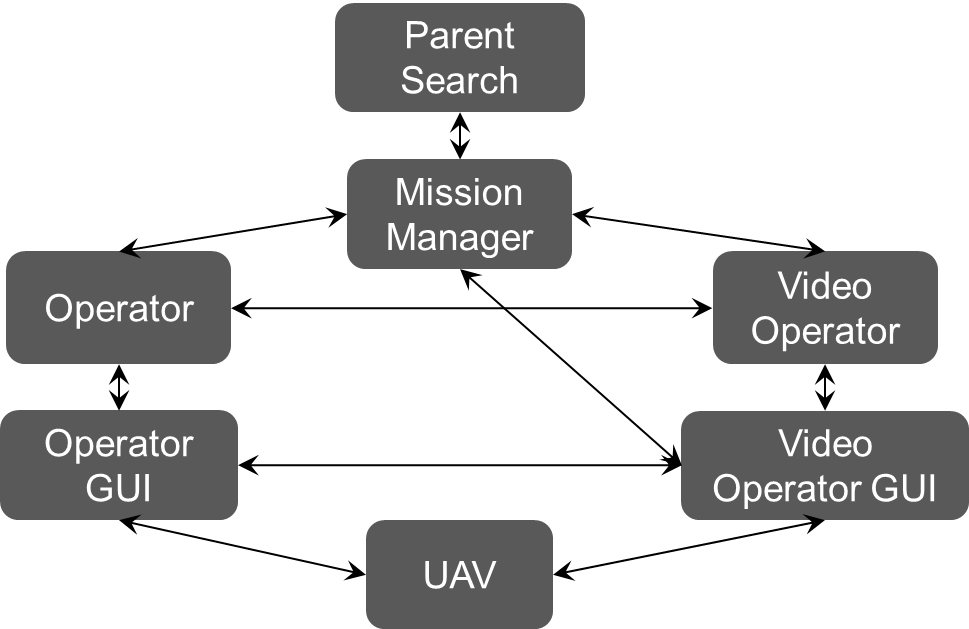
\includegraphics[height=2in]{ditg.png}
\caption{High Level DiTG}
\label{fig:ditg}
\end{figure}

\begin{figure}
\center
\setlength{\abovecaptionskip}{1mm}
\setlength{\belowcaptionskip}{1mm}
\setlength{\textfloatsep}{1mm}
\setlength{\floatsep}{1mm}
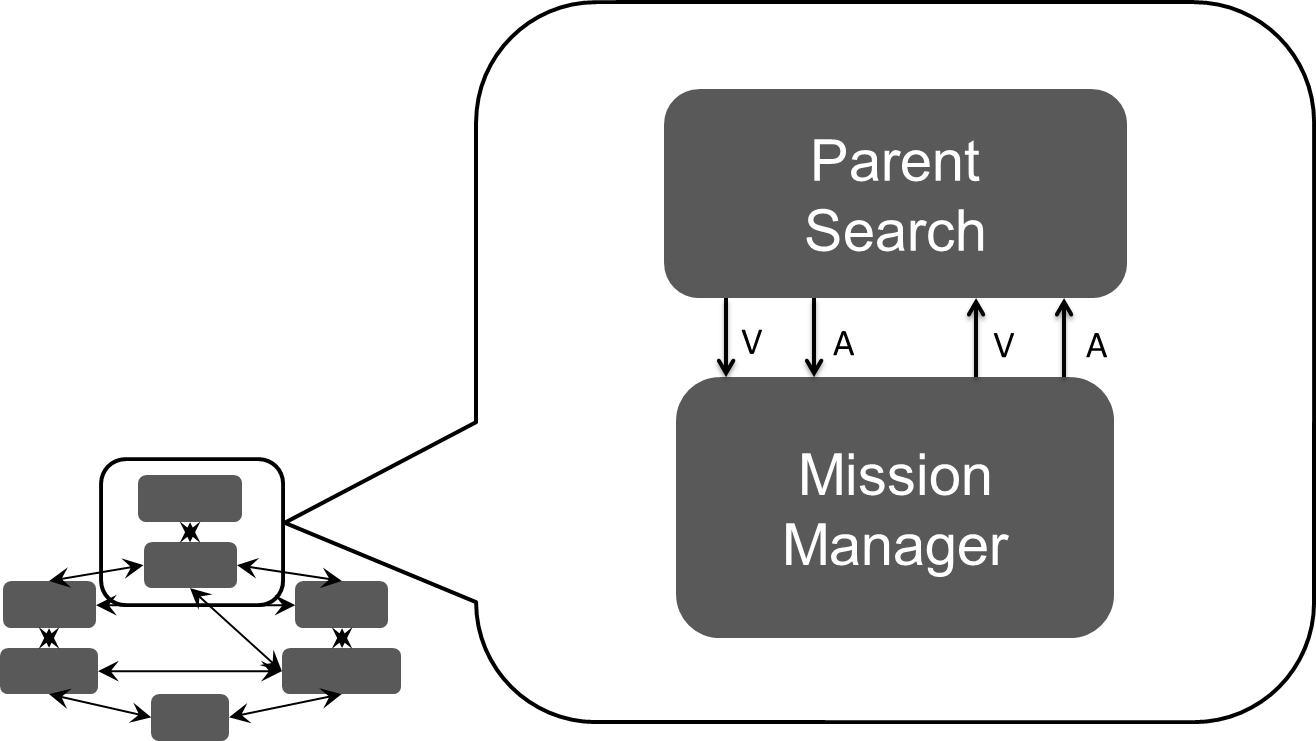
\includegraphics[height=1.9in]{ditg_detailed.png}
\caption{Detail view of DiTG: V is a Visual channel and A is an Audio channel}
\label{fig:ditg_detail}
\end{figure}

Formally, the models are the following mathematical structures:
 \begin{equation}
 	DiTG = (A, \Phi, \forall a_i \in A~ \exists \Phi_i \subset \Phi)
 \end{equation}

 \begin{equation}
 	Actor = (S, s_0, s_{current}, \Omega_A, \Sigma_A \subset \Phi, \Lambda_A
 	\subset \Phi)
 \label{eq:actor}
 \end{equation}

 \begin{equation}
	State = (T_{enabled}, T_{disabled})
 \label{eq:state}
\end{equation}

\begin{equation}
\begin{split}
	Transition = (\Omega_{input} \subset \Omega_A, \Sigma_{input} \subset \Sigma_A,\\
	\Omega_{value}^{input}, \Sigma_{value}^{input} \\
	\Omega_{output} \subset \Omega_A, \Lambda_{output} \subset \Lambda_A, \\
	\Omega_{value}^{output}, \Lambda_{value}^{output})
 \label{eq:transition}
 \end{split}
\end{equation}

\begin{equation}
\begin{split}
Channel (\phi) = (type \in (visual, audio), \\
value \in (null, *), 
 a_i^{source}, a_j^{target}) : i \neq j
 \label{eq:channel}
 \end{split}
\end{equation}

\begin{equation}
Declarative Memory(\omega) = value \in (null, *)
\end{equation}


where $A$ is a set of actors, $S$ a set of
states, $T$ a set of transitions, $\Phi$ a set of channels, $\Omega$ a set of
declarative memory, $\Sigma$ a set of input channels, and $\Lambda$ a set of
output channels.

\subsection{Framework Components}
\subsubsection{Actors}
Actors represent the agents within the system, while an Actor may be any type of agent for the context of workload we assume that an Actor is human.  An Actor is made up of a current state, the set of all possible states, declarative memory, and channels and are represented within the model as finite state machines.

\subsubsection{States}
States contain a set of all possible transitions to other Actor states.  While states typically represent the performance of a set of tasks they can also represent such things as emotion, fatigue, and neglect which is expressed in the transitions.  In this way an Actor�s current state represents its current decision making paradigm.

\subsubsection{Transitions}
A transition is composed of a set of required declarative memory and channel values, a set of declarative memory and channel output values, an end state, and a duration.  A transition is considered enabled when all of its input requirements are met.  The duration represents the relative difficulty of the task(s) associated with the transition.  We rationalize this by assuming that all tasks are performed at a constant rate, thus more difficult tasks take longer.

\subsubsection{Declarative Memory }
This memory represents internal facts stored by an Actor and used in decision making.  This memory takes the form of internal variables within an Actor, transitions can look for specific values on these variables to determine if they are enabled.

\subsubsection{Channels} 
Channels represent physical communication mediums that exist between Actors.  Each channel has a type (audio or visual), a buffer, a source, and a target.  The channel type is associated with the modality dimension of multiple resource theory while the source and target represent the stages dimension.  The source being the response and the target being perception/cognition.  We assume that all channels have a constant bandwidth, the longer a channel is in use the more data being sent across the channel.

\subsubsection{How it works}
We represent a system as a directed team graph (DiTG).  This is a collection of Actors connected to one another by a set of channels.  Whenever the state of the system changes an Actor will petition, from its current state, a list of enabled transitions thus defining what decisions can be made.  The Actor may then activate one of these transitions.  Transitions have two main states, active and fired.  When chosen a transition is made active, after the specified duration the transition fires.  When a transition becomes active it creates temporary output values for declarative memory and channels.  These temporary values are then applied to the actual declarative memory and channels when the transition fires.  

\subsection{Actor vs Tasks}
This architecture focuses on the Actor itself and less on the tasks performed by the Actor.  The difference being that Actor states can account for conditions on the Actor which affect performance and increase workload which cannot be seen simply by taking a set of tasks and examining their combined resource requirements.  For our model we never explicitly define a single task.  Instead we define Actors, States, and Transitions.  Each transition defines its own perceptual, cognitive, response, and declarative resources (Salvucci) which are not restricted to performing a single task.  The state contains all the possible transitions an Actor can choose from given its current state representing the performance of multiple tasks and procedural resources.  The Actor acts as the final cognitive resource by choosing which transition to follow.  In this way we achieve multi-tasking not by defining specific tasks but by defining the choices an Actor can make and the resources affected by each choice.
